% Drawing 154/02-15 -- folder 154, batch 02, archive page 38 (PDF page 39).
% Transcription: figure, en haut de la moitié droite : quatre disques au bord vert, traversés de cordes orange (pleines et pointillées), accolés deux à deux en quatre points de contact (petits segments foncés), autour d'un domaine central bordé d'arcs bruns ; les extrémités des cordes sont marquées $D_0$, $D'_0$, $D_1$, $D'_1$, et les coins voisins des contacts portent les lettres $\alpha$, $\beta$, $\beta'$
% Kind: four chord systems in disks glued around a central domain. Method 2 (schematic redraw from the facsimile). Status: partial.
% Notes: Top of the right half: four disks with green rims crossed by orange chords (solid and dotted), glued two by two at four contact points (short dark segments), around a central domain bounded by brown arcs; the chord ends marked D_0, D'_0, D_1, D'_1, and the corners next to the contacts lettered alpha, beta, beta' (placed approximately). Disks, contacts and labels placed from the crop; the chords and the orange wedges are schematic.
% Coordinates: 1 unit = 1 mm = 1/100 of the crop width (bbox in page fractions: [0.556, 0.095, 0.814, 0.278]).
% Redrawn by Claude (claude-opus-5-5), issue #73, 2026-11-07; not checked by a human; not compiled (no TeX in the session).
% Rights: reproduces part of the work -- behind RENDER_TRANSCRIPTS, never published by itself.
\documentclass[tikz,border=3pt]{standalone}
\usepackage{amsmath,amssymb}
\usetikzlibrary{patterns,arrows.meta}
\tikzset{Or/.style={orange!90!black}, Ye/.style={yellow!80!orange}, Lg/.style={green!60!black!70}, Dg/.style={green!45!black}, Br/.style={brown!80!black}, Rd/.style={red!85!black}, Bl/.style={blue!70!black}, Gy/.style={black!40}, pencil/.style={black!45}, struck/.style={black!35}, mark/.style={circle,draw,inner sep=1.3pt}, pt/.style={circle,fill,inner sep=0.9pt}, opt/.style={circle,draw,fill=white,inner sep=1.1pt}}
\begin{document}
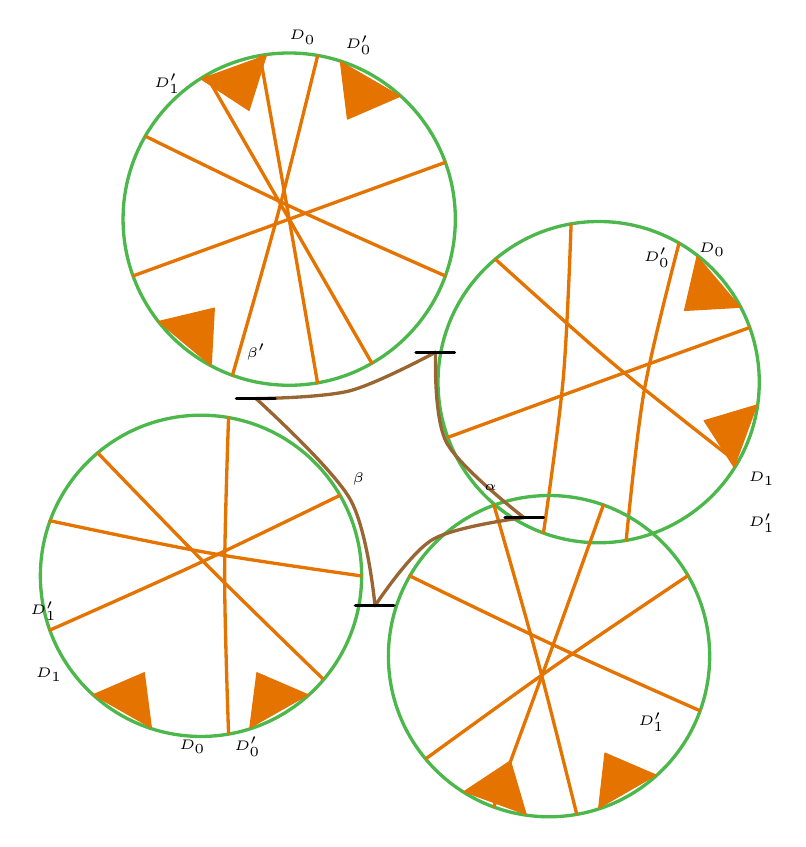
\begin{tikzpicture}[x=1mm,y=1mm,line cap=round,line join=round,font=\scriptsize]
\draw[Lg,very thick] (34.4,-27.7) ellipse[x radius=21.1, y radius=21.1];
\draw[Or,very thick] plot[smooth, tension=0.55] coordinates {(30.7,-7) (34.4,-27.7) (38,-48.5)};
\draw[Or,very thick] plot[smooth, tension=0.55] coordinates {(23.9,-9.5) (34.4,-27.7) (44.9,-46)};
\draw[Or,very thick] plot[smooth, tension=0.55] coordinates {(38,-7) (32.9,-27.3) (27.2,-47.5)};
\draw[Or,very thick] plot[smooth, tension=0.55] coordinates {(16.2,-17.2) (35,-26.3) (54.2,-34.9)};
\draw[Or,very thick] plot[smooth, tension=0.55] coordinates {(14.6,-34.9) (34.4,-27.7) (54.2,-20.5)};
\draw[Or] (31.5,-6.9) -- (23.2,-9.9) -- (29.3,-13.9) -- cycle;
\fill[pattern=north east lines,Or] (31.5,-6.9) -- (23.2,-9.9) -- (29.3,-13.9) -- cycle;
\draw[Or] (48.5,-12.1) -- (40.9,-7.7) -- (41.8,-15) -- cycle;
\fill[pattern=north east lines,Or] (48.5,-12.1) -- (40.9,-7.7) -- (41.8,-15) -- cycle;
\draw[Or] (17.8,-40.7) -- (24.5,-46.3) -- (24.9,-39) -- cycle;
\fill[pattern=north east lines,Or] (17.8,-40.7) -- (24.5,-46.3) -- (24.9,-39) -- cycle;
\draw[Lg,very thick] (73.7,-48.4) ellipse[x radius=20.4, y radius=20.4];
\draw[Or,very thick] plot[smooth, tension=0.55] coordinates {(70.2,-28.4) (69.2,-48) (66.7,-67.5)};
\draw[Or,very thick] plot[smooth, tension=0.55] coordinates {(60.6,-32.8) (75.6,-46.1) (91.3,-58.6)};
\draw[Or,very thick] plot[smooth, tension=0.55] coordinates {(92.8,-41.5) (73.7,-48.4) (54.6,-55.4)};
\draw[Or,very thick] plot[smooth, tension=0.55] coordinates {(83.9,-30.8) (79.5,-49.4) (77.2,-68.5)};
\draw[Or] (91.7,-38.9) -- (86.2,-32.4) -- (84.6,-39.3) -- cycle;
\fill[pattern=north east lines,Or] (91.7,-38.9) -- (86.2,-32.4) -- (84.6,-39.3) -- cycle;
\draw[Or] (90.9,-59.2) -- (93.8,-51.3) -- (87.1,-53.3) -- cycle;
\fill[pattern=north east lines,Or] (90.9,-59.2) -- (93.8,-51.3) -- (87.1,-53.3) -- cycle;
\draw[Lg,very thick] (23.2,-73) ellipse[x radius=20.4, y radius=20.4];
\draw[Or,very thick] plot[smooth, tension=0.55] coordinates {(26.7,-52.9) (26.2,-73) (26.7,-93)};
\draw[Or,very thick] plot[smooth, tension=0.55] coordinates {(4,-66) (23.7,-70) (43.5,-73)};
\draw[Or,very thick] plot[smooth, tension=0.55] coordinates {(10.1,-57.4) (24.2,-71.9) (38.7,-86.1)};
\draw[Or,very thick] plot[smooth, tension=0.55] coordinates {(4,-79.9) (22.5,-71.6) (40.8,-62.8)};
\draw[Or] (9.5,-88.1) -- (16.9,-92.3) -- (16,-85.3) -- cycle;
\fill[pattern=north east lines,Or] (9.5,-88.1) -- (16.9,-92.3) -- (16,-85.3) -- cycle;
\draw[Or] (29.4,-92.3) -- (36.8,-88.1) -- (30.3,-85.3) -- cycle;
\fill[pattern=north east lines,Or] (29.4,-92.3) -- (36.8,-88.1) -- (30.3,-85.3) -- cycle;
\draw[Lg,very thick] (67.4,-83.2) ellipse[x radius=20.4, y radius=20.4];
\draw[Or,very thick] plot[smooth, tension=0.55] coordinates {(60.4,-64) (65.9,-83.5) (70.9,-103.2)};
\draw[Or,very thick] plot[smooth, tension=0.55] coordinates {(49.7,-73) (68,-81.8) (86.5,-90.1)};
\draw[Or,very thick] plot[smooth, tension=0.55] coordinates {(85,-73) (68.2,-84.4) (51.8,-96.2)};
\draw[Or,very thick] plot[smooth, tension=0.55] coordinates {(74.3,-64) (67.4,-83.2) (60.4,-102.3)};
\draw[Or] (73.7,-102.5) -- (81,-98.3) -- (74.5,-95.5) -- cycle;
\fill[pattern=north east lines,Or] (73.7,-102.5) -- (81,-98.3) -- (74.5,-95.5) -- cycle;
\draw[Or] (56.6,-100.4) -- (64.5,-103.3) -- (62.5,-96.5) -- cycle;
\fill[pattern=north east lines,Or] (56.6,-100.4) -- (64.5,-103.3) -- (62.5,-96.5) -- cycle;
\draw[Br,very thick] plot[smooth, tension=0.55] coordinates {(30.2,-50.5) (42.1,-49.5) (53,-44.6)};
\draw[Br,very thick] plot[smooth, tension=0.55] coordinates {(53,-44.6) (54.4,-56.1) (64.2,-65.6)};
\draw[Br,very thick] plot[smooth, tension=0.55] coordinates {(64.2,-65.6) (52.6,-68.4) (45.3,-76.8)};
\draw[Br,very thick] plot[smooth, tension=0.55] coordinates {(45.3,-76.8) (42.1,-63.2) (30.2,-50.5)};
\draw[very thick] (27.7,-50.5) -- (32.6,-50.5);
\draw[very thick] (50.5,-44.6) -- (55.4,-44.6);
\draw[very thick] (61.8,-65.6) -- (66.7,-65.6);
\draw[very thick] (42.8,-76.8) -- (47.7,-76.8);
\node[inner sep=1pt] at (18.9,-10.5) {\tiny $D'_1$};
\node[inner sep=1pt] at (36.1,-4.6) {\tiny $D_0$};
\node[inner sep=1pt] at (43.2,-5.6) {\tiny $D'_0$};
\node[inner sep=1pt] at (81.1,-32.6) {\tiny $D'_0$};
\node[inner sep=1pt] at (88.1,-31.6) {\tiny $D_0$};
\node[inner sep=1pt] at (94.4,-60.7) {\tiny $D_1$};
\node[inner sep=1pt] at (94.4,-66.3) {\tiny $D'_1$};
\node[inner sep=1pt] at (3.2,-77.5) {\tiny $D'_1$};
\node[inner sep=1pt] at (3.9,-85.6) {\tiny $D_1$};
\node[inner sep=1pt] at (22.1,-94.7) {\tiny $D_0$};
\node[inner sep=1pt] at (29.1,-94.7) {\tiny $D'_0$};
\node[inner sep=1pt] at (80.4,-91.6) {\tiny $D'_1$};
\node[inner sep=1pt] at (60,-61.8) {\tiny $\alpha$};
\node[inner sep=1pt] at (43.2,-60.7) {\tiny $\beta$};
\node[inner sep=1pt] at (30.2,-44.6) {\tiny $\beta'$};
\end{tikzpicture}
\end{document}
